\chapter{The project and my mission}

This chapter will introduce the project I was assigned, and the mission I was given.

\section{The project}

This new project involves designing an autonomus navigation algorithm for a robot, which will be moving in an unknown environment. 

~~

A robot is a machine that can do the work of a person, automatically or by being controlled (i.e. a computer or a person). In this project, a robot is defined as a mechanical device that has wheels allowing it to move freely in his surrounding.In order to detect and take note of the surroundings, it is also required that the robot is equiped with cameras ans sensors. Those sensors will provide additionnal information, such as depth, height, or spacial position (x, y, z). 
As for now, the \gls{UPES} doesn't have the robot for the moment. 

~~

The robot will have to move in an environment from a position to another. Both of those two positions are known, but the path to take in order to move from one to another is not. Obstacles could be found in this environment (i.e. everything that could be on the way of the robot and block it, like rocks, walls or holes in the ground). 

~~

In general, navigation can be divided into two parts, whether it is performed in a knowned or an unknowned enviromnent. They differ by the knowleadge about the environment the agent possess (the robot) \cite{Russell:2010:AIM} : 
\begin{description}
	\item[Known environment] the agent know the outcome of every action it can take. For a robot, it means that it knows the path to take and all obstacle's positions it can encounter in advance 
	\item[Unknown environment] the agent doesn't know the outcome of every action, and have to learn from his previous actions in order to make good decisions. For a robot, it means that the robot doesn't know the obstacle's position in advance, nor the path to take.
\end{description}
In our case, the robot will explore in an unknown environment, for example it could explore and search into a submarin field, or the planet Mars. 

~~

So as to navigate correctly, a 3-Dimension map will be generated using at least two cameras. The different objects present on this map will be recognized and tagged as to whether they are obstacles or not. A depth map could be used in order to generate the 3D map from two images (i.e. left and right images). Today's 3D map generation technics generally use \gls{DIP} algorithms, but regarding this project, symbolic computing algorithms will be used, as it has been shown in recent research papers that this technic is computing faster than nowadays other algorithms. \Gls{DIP} and symbolic computing are transformations, \gls{image processing} algorithms. % Symbolic computing is a transformation (an image processing) using symbols. 

~~ 

Autonomous navigation means that the robot will have to navigate from it's own, without help and automatically. \gls{AI} will be an essential part of this process. Multiples \gls{AI} algorithms exist, like A$^*$, D$^*$, Swarm Intelligence, \gls{PSO}, Hill Climbing, and Genetic Algorithm. As the robot will navigate in an unknown environment, it is necessary that the robot learn from his previous decisions. In order to do that, a reinforcement learning will be used, which will allow the robot to self-learning through his experiences and a reward policy.  


~~

The \vref{fig:general functionning} shows the general functionning of the robot. This project will be devided into three parts : 
\begin{description}
	\item[3D Map Generation] this part involves processing the images taken by the cameras, reducing the noise, generating the 3D map from (at least) two images and identifying the obstacles (by tagging the 3D map)
	\item[Navigation Part] in this part, the navigation algorithm will be implemented, and will use the tagged 3D map
	\item[\gls{AI} Part] the last part is related to the implementation of a reinforcement learning algorithm through a reward policy
\end{description}


\begin{figure}[H]
	\centering
	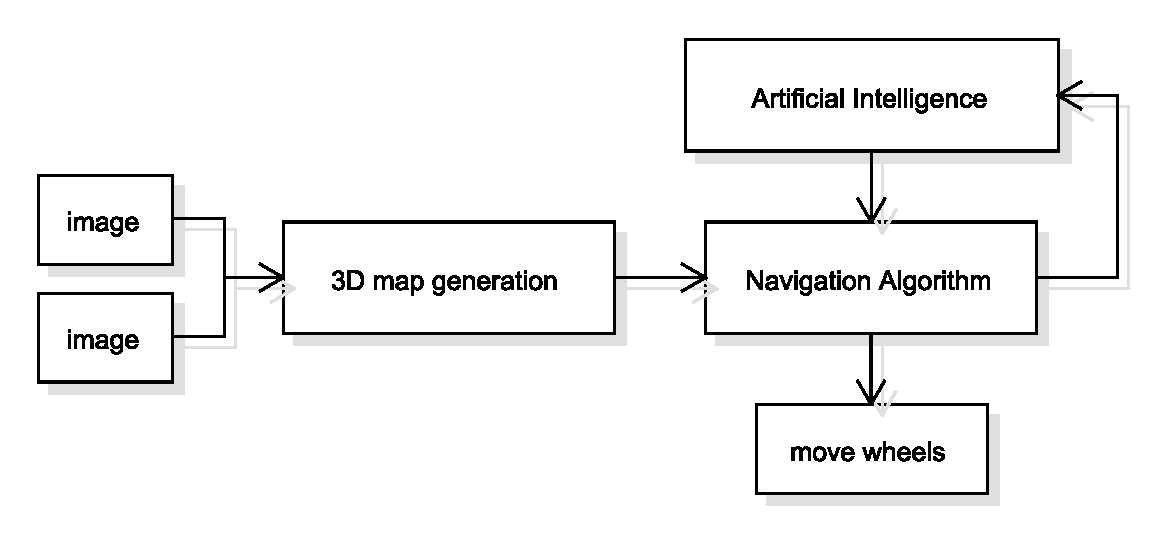
\includegraphics[width=0.6\textwidth]{images/diagrams/flowchart_general}	
    \caption{General functionning}
    \label{fig:general functionning}
\end{figure}



~~

In other words, the objective of the reseach is "To design and develop a self-learning algorithm for an autonomous moving system equipped with 3D vision technique" \cite{bib:niharika}.



\section{My mission in this project}

objectif 
contrainte 
attente 

\gls{GUI}

